% GNUPLOT: LaTeX picture with Postscript
\begingroup
  \makeatletter
  \providecommand\color[2][]{%
    \GenericError{(gnuplot) \space\space\space\@spaces}{%
      Package color not loaded in conjunction with
      terminal option `colourtext'%
    }{See the gnuplot documentation for explanation.%
    }{Either use 'blacktext' in gnuplot or load the package
      color.sty in LaTeX.}%
    \renewcommand\color[2][]{}%
  }%
  \providecommand\includegraphics[2][]{%
    \GenericError{(gnuplot) \space\space\space\@spaces}{%
      Package graphicx or graphics not loaded%
    }{See the gnuplot documentation for explanation.%
    }{The gnuplot epslatex terminal needs graphicx.sty or graphics.sty.}%
    \renewcommand\includegraphics[2][]{}%
  }%
  \providecommand\rotatebox[2]{#2}%
  \@ifundefined{ifGPcolor}{%
    \newif\ifGPcolor
    \GPcolorfalse
  }{}%
  \@ifundefined{ifGPblacktext}{%
    \newif\ifGPblacktext
    \GPblacktexttrue
  }{}%
  % define a \g@addto@macro without @ in the name:
  \let\gplgaddtomacro\g@addto@macro
  % define empty templates for all commands taking text:
  \gdef\gplbacktext{}%
  \gdef\gplfronttext{}%
  \makeatother
  \ifGPblacktext
    % no textcolor at all
    \def\colorrgb#1{}%
    \def\colorgray#1{}%
  \else
    % gray or color?
    \ifGPcolor
      \def\colorrgb#1{\color[rgb]{#1}}%
      \def\colorgray#1{\color[gray]{#1}}%
      \expandafter\def\csname LTw\endcsname{\color{white}}%
      \expandafter\def\csname LTb\endcsname{\color{black}}%
      \expandafter\def\csname LTa\endcsname{\color{black}}%
      \expandafter\def\csname LT0\endcsname{\color[rgb]{1,0,0}}%
      \expandafter\def\csname LT1\endcsname{\color[rgb]{0,1,0}}%
      \expandafter\def\csname LT2\endcsname{\color[rgb]{0,0,1}}%
      \expandafter\def\csname LT3\endcsname{\color[rgb]{1,0,1}}%
      \expandafter\def\csname LT4\endcsname{\color[rgb]{0,1,1}}%
      \expandafter\def\csname LT5\endcsname{\color[rgb]{1,1,0}}%
      \expandafter\def\csname LT6\endcsname{\color[rgb]{0,0,0}}%
      \expandafter\def\csname LT7\endcsname{\color[rgb]{1,0.3,0}}%
      \expandafter\def\csname LT8\endcsname{\color[rgb]{0.5,0.5,0.5}}%
    \else
      % gray
      \def\colorrgb#1{\color{black}}%
      \def\colorgray#1{\color[gray]{#1}}%
      \expandafter\def\csname LTw\endcsname{\color{white}}%
      \expandafter\def\csname LTb\endcsname{\color{black}}%
      \expandafter\def\csname LTa\endcsname{\color{black}}%
      \expandafter\def\csname LT0\endcsname{\color{black}}%
      \expandafter\def\csname LT1\endcsname{\color{black}}%
      \expandafter\def\csname LT2\endcsname{\color{black}}%
      \expandafter\def\csname LT3\endcsname{\color{black}}%
      \expandafter\def\csname LT4\endcsname{\color{black}}%
      \expandafter\def\csname LT5\endcsname{\color{black}}%
      \expandafter\def\csname LT6\endcsname{\color{black}}%
      \expandafter\def\csname LT7\endcsname{\color{black}}%
      \expandafter\def\csname LT8\endcsname{\color{black}}%
    \fi
  \fi
    \setlength{\unitlength}{0.0500bp}%
    \ifx\gptboxheight\undefined%
      \newlength{\gptboxheight}%
      \newlength{\gptboxwidth}%
      \newsavebox{\gptboxtext}%
    \fi%
    \setlength{\fboxrule}{0.5pt}%
    \setlength{\fboxsep}{1pt}%
\begin{picture}(7200.00,5040.00)%
    \gplgaddtomacro\gplbacktext{%
      \csname LTb\endcsname%
      \put(946,920){\makebox(0,0)[r]{\strut{}0 }}%
      \csname LTb\endcsname%
      \put(946,1691){\makebox(0,0)[r]{\strut{}50k}}%
      \csname LTb\endcsname%
      \put(946,2462){\makebox(0,0)[r]{\strut{}100k}}%
      \csname LTb\endcsname%
      \put(946,3233){\makebox(0,0)[r]{\strut{}150k}}%
      \csname LTb\endcsname%
      \put(946,4004){\makebox(0,0)[r]{\strut{}200k}}%
      \csname LTb\endcsname%
      \put(946,4775){\makebox(0,0)[r]{\strut{}250k}}%
      \put(1141,725){\rotatebox{-45}{\makebox(0,0)[l]{\strut{}$0$}}}%
      \put(1367,725){\rotatebox{-45}{\makebox(0,0)[l]{\strut{}$40$}}}%
      \put(1594,725){\rotatebox{-45}{\makebox(0,0)[l]{\strut{}$80$}}}%
      \put(1820,725){\rotatebox{-45}{\makebox(0,0)[l]{\strut{}$120$}}}%
      \put(2047,725){\rotatebox{-45}{\makebox(0,0)[l]{\strut{}$160$}}}%
      \put(2273,725){\rotatebox{-45}{\makebox(0,0)[l]{\strut{}$200$}}}%
      \put(2500,725){\rotatebox{-45}{\makebox(0,0)[l]{\strut{}$240$}}}%
      \put(2726,725){\rotatebox{-45}{\makebox(0,0)[l]{\strut{}$280$}}}%
      \put(2953,725){\rotatebox{-45}{\makebox(0,0)[l]{\strut{}$320$}}}%
      \put(3179,725){\rotatebox{-45}{\makebox(0,0)[l]{\strut{}$360$}}}%
      \put(3406,725){\rotatebox{-45}{\makebox(0,0)[l]{\strut{}$400$}}}%
      \put(3632,725){\rotatebox{-45}{\makebox(0,0)[l]{\strut{}$440$}}}%
      \put(3859,725){\rotatebox{-45}{\makebox(0,0)[l]{\strut{}$480$}}}%
      \put(4085,725){\rotatebox{-45}{\makebox(0,0)[l]{\strut{}$520$}}}%
      \put(4312,725){\rotatebox{-45}{\makebox(0,0)[l]{\strut{}$560$}}}%
      \put(4538,725){\rotatebox{-45}{\makebox(0,0)[l]{\strut{}$600$}}}%
      \put(4765,725){\rotatebox{-45}{\makebox(0,0)[l]{\strut{}$640$}}}%
      \put(4991,725){\rotatebox{-45}{\makebox(0,0)[l]{\strut{}$680$}}}%
      \put(5218,725){\rotatebox{-45}{\makebox(0,0)[l]{\strut{}$720$}}}%
      \put(5444,725){\rotatebox{-45}{\makebox(0,0)[l]{\strut{}$760$}}}%
      \put(5671,725){\rotatebox{-45}{\makebox(0,0)[l]{\strut{}$800$}}}%
      \put(5897,725){\rotatebox{-45}{\makebox(0,0)[l]{\strut{}$840$}}}%
      \put(6124,725){\rotatebox{-45}{\makebox(0,0)[l]{\strut{}$880$}}}%
      \put(6350,725){\rotatebox{-45}{\makebox(0,0)[l]{\strut{}$920$}}}%
      \put(6577,725){\rotatebox{-45}{\makebox(0,0)[l]{\strut{}$960$}}}%
      \put(6803,725){\rotatebox{-45}{\makebox(0,0)[l]{\strut{}$1000$}}}%
    }%
    \gplgaddtomacro\gplfronttext{%
      \csname LTb\endcsname%
      \put(176,2847){\rotatebox{-270}{\makebox(0,0){\strut{}Number of responses}}}%
      \put(3972,154){\makebox(0,0){\strut{}Response times in ms}}%
      \put(3972,4665){\makebox(0,0){\strut{}}}%
    }%
    \gplbacktext
    \put(0,0){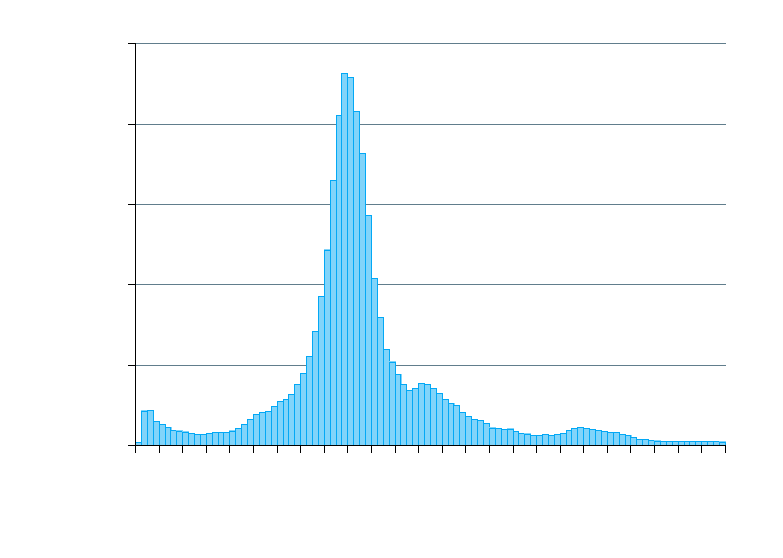
\includegraphics{resp_dist_heavy}}%
    \gplfronttext
  \end{picture}%
\endgroup
